%% LyX 2.3.5.2 created this file.  For more info, see http://www.lyx.org/.
%% Do not edit unless you really know what you are doing.
\documentclass[11pt,english,openright]{book}
\usepackage[T1]{fontenc}
\usepackage[latin9]{inputenc}
\usepackage[a4paper]{geometry}
\geometry{verbose,tmargin=3cm,bmargin=3.5cm,lmargin=4cm,rmargin=3cm}
\setcounter{secnumdepth}{3}
\setcounter{tocdepth}{3}
\usepackage{color}
\usepackage{babel}
\usepackage{float}
\usepackage{booktabs}
\usepackage{url}
\usepackage{amsmath}
\usepackage{amssymb}
\usepackage{graphicx}
\usepackage{setspace}
\onehalfspacing
\usepackage[unicode=true,pdfusetitle,
 bookmarks=true,bookmarksnumbered=false,bookmarksopen=false,
 breaklinks=false,pdfborder={0 0 1},backref=false,colorlinks=false]
 {hyperref}

\makeatletter

%%%%%%%%%%%%%%%%%%%%%%%%%%%%%% LyX specific LaTeX commands.
\providecommand{\LyX}{\texorpdfstring%
  {L\kern-.1667em\lower.25em\hbox{Y}\kern-.125emX\@}
  {LyX}}
\DeclareRobustCommand*{\lyxarrow}{%
\@ifstar
{\leavevmode\,$\triangleleft$\,\allowbreak}
{\leavevmode\,$\triangleright$\,\allowbreak}}
%% Because html converters don't know tabularnewline
\providecommand{\tabularnewline}{\\}
\floatstyle{ruled}
\newfloat{algorithm}{tbp}{loa}[chapter]
\providecommand{\algorithmname}{Algorithm}
\floatname{algorithm}{\protect\algorithmname}

%%%%%%%%%%%%%%%%%%%%%%%%%%%%%% User specified LaTeX commands.
% additional packages
\usepackage{tabularx}
\usepackage{setspace}
\usepackage{amsthm}
\usepackage{rotating}
\usepackage{caption}
\usepackage{epsfig}
\usepackage{indentfirst}
\usepackage{fancyhdr}
\usepackage{url}
\usepackage{cite}
\usepackage[normalem]{ulem}
\usepackage[table]{xcolor}
\usepackage{booktabs}
\usepackage{algpseudocode}

% this is a dirty fix for LTS version of Ubuntu/Kubuntu that has a
% very outdated "geometry" package
%%
%% This is file `geometry.sty',
%% generated with the docstrip utility.
%%
%% The original source files were:
%%
%% geometry.dtx  (with options: `package')
%% 
%% Copyright (C) 1996-2010
%% by Hideo Umeki <latexgeometry@gmail.com>
%% 
%% This work may be distributed and/or modified under the conditions of
%% the LaTeX Project Public License, either version 1.3c of this license
%% or (at your option) any later version. The latest version of this
%% license is in
%%    http://www.latex-project.org/lppl.txt
%% and version 1.3c or later is part of all distributions of LaTeX
%% version 2005/12/01 or later.
%% 
%% This work is "maintained" (as per the LPPL maintenance status)
%% by Hideo Umeki.
%% 
%% This work consists of the files geometry.dtx and
%% the derived files: geometry.{sty,ins,drv}, geometry-samples.tex.
%% 
\NeedsTeXFormat{LaTeX2e}
\ProvidesPackage{geometry}
  [2010/09/12 v5.6 Page Geometry]
\RequirePackage{keyval}%
\RequirePackage{ifpdf}%
\RequirePackage{ifvtex}%
\RequirePackage{ifxetex}%
\newif\ifGm@verbose
\newif\ifGm@landscape
\newif\ifGm@swap@papersize
\newif\ifGm@includehead
\newif\ifGm@includefoot
\newif\ifGm@includemp
\newif\ifGm@hbody
\newif\ifGm@vbody
\newif\ifGm@heightrounded
\newif\ifGm@showframe
\newif\ifGm@showcrop
\newif\ifGm@pass
\newif\ifGm@resetpaper
\newif\ifGm@layout
\newif\ifGm@newgm
\newcount\Gm@cnth
\newcount\Gm@cntv
\newcount\c@Gm@tempcnt
\newdimen\Gm@bindingoffset
\newdimen\Gm@wd@mp
\newdimen\Gm@odd@mp
\newdimen\Gm@even@mp
\newdimen\Gm@layoutwidth
\newdimen\Gm@layoutheight
\newdimen\Gm@layouthoffset
\newdimen\Gm@layoutvoffset
\newtoks\Gm@dimlist
\def\Gm@warning#1{\PackageWarningNoLine{geometry}{#1}}%
\def\ifGm@preamble#1{%
  \ifGm@newgm
   \Gm@warning{`#1': not available in `\string\newgeometry'; skipped}%
  \else
    \expandafter\@firstofone
  \fi}%
\def\Gm@Dhratio{1:1}% = left:right default for oneside
\def\Gm@Dhratiotwo{2:3}% = inner:outer default for twoside.
\def\Gm@Dvratio{2:3}% = top:bottom default
\def\Gm@Dhscale{0.7}%
\def\Gm@Dvscale{0.7}%
\def\Gm@dvips{dvips}%
\def\Gm@dvipdfm{dvipdfm}%
\def\Gm@pdftex{pdftex}%
\def\Gm@xetex{xetex}%
\def\Gm@vtex{vtex}%
\def\Gm@true{true}%
\def\Gm@false{false}%
\edef\Gm@orgpw{\the\paperwidth}%
\edef\Gm@orgph{\the\paperheight}%
\def\Gm@savelength#1{%
  \g@addto@macro\Gm@restore{\expandafter\noexpand\expandafter\csname
  #1\endcsname\expandafter=\expandafter\the\csname #1\endcsname\relax}}%
\def\Gm@saveboolean#1{%
  \csname if#1\endcsname
    \g@addto@macro\Gm@restore{\expandafter\noexpand\csname #1true\endcsname}%
  \else
    \g@addto@macro\Gm@restore{\expandafter\noexpand\csname #1false\endcsname}%
  \fi}%
\def\Gm@restore{}%
\def\Gm@save{%
  \Gm@savelength{paperwidth}%
  \Gm@savelength{paperheight}%
  \Gm@savelength{textwidth}%
  \Gm@savelength{textheight}%
  \Gm@savelength{evensidemargin}%
  \Gm@savelength{oddsidemargin}%
  \Gm@savelength{topmargin}%
  \Gm@savelength{headheight}%
  \Gm@savelength{headsep}%
  \Gm@savelength{topskip}%
  \Gm@savelength{footskip}%
  \Gm@savelength{baselineskip}%
  \Gm@savelength{marginparwidth}%
  \Gm@savelength{marginparsep}%
  \Gm@savelength{columnsep}%
  \Gm@savelength{hoffset}%
  \Gm@savelength{voffset}
  \Gm@savelength{Gm@layoutwidth}%
  \Gm@savelength{Gm@layoutheight}%
  \Gm@savelength{Gm@layouthoffset}%
  \Gm@savelength{Gm@layoutvoffset}%
  \Gm@saveboolean{@twocolumn}%
  \Gm@saveboolean{@twoside}%
  \Gm@saveboolean{@mparswitch}%
  \Gm@saveboolean{@reversemargin}}%
\def\Gm@initnewgm{%
  \Gm@passfalse
  \Gm@swap@papersizefalse
  \Gm@dimlist={}
  \Gm@hbodyfalse
  \Gm@vbodyfalse
  \Gm@heightroundedfalse
  \Gm@includeheadfalse
  \Gm@includefootfalse
  \Gm@includempfalse
  \let\Gm@width\@undefined
  \let\Gm@height\@undefined
  \let\Gm@textwidth\@undefined
  \let\Gm@textheight\@undefined
  \let\Gm@lines\@undefined
  \let\Gm@hscale\@undefined
  \let\Gm@vscale\@undefined
  \let\Gm@hmarginratio\@undefined
  \let\Gm@vmarginratio\@undefined
  \let\Gm@lmargin\@undefined
  \let\Gm@rmargin\@undefined
  \let\Gm@tmargin\@undefined
  \let\Gm@bmargin\@undefined
  \Gm@layoutfalse
  \Gm@layouthoffset\z@
  \Gm@layoutvoffset\z@
  \Gm@bindingoffset\z@}%
\def\Gm@initall{%
  \let\Gm@driver\@empty
  \let\Gm@truedimen\@empty
  \let\Gm@paper\@undefined
  \Gm@resetpaperfalse
  \Gm@landscapefalse
  \Gm@verbosefalse
  \Gm@showframefalse
  \Gm@showcropfalse
  \Gm@newgmfalse
  \Gm@initnewgm}%
\def\Gm@setdriver#1{%
  \expandafter\let\expandafter\Gm@driver\csname Gm@#1\endcsname}%
\def\Gm@unsetdriver#1{%
  \expandafter\ifx\csname Gm@#1\endcsname\Gm@driver\let\Gm@driver\@empty\fi}%
\def\Gm@setbool{\@dblarg\Gm@@setbool}%
\def\Gm@setboolrev{\@dblarg\Gm@@setboolrev}%
\def\Gm@@setbool[#1]#2#3{\Gm@doif{#1}{#3}{\csname Gm@#2\Gm@bool\endcsname}}%
\def\Gm@@setboolrev[#1]#2#3{\Gm@doifelse{#1}{#3}%
  {\csname Gm@#2\Gm@false\endcsname}{\csname Gm@#2\Gm@true\endcsname}}%
\def\Gm@doif#1#2#3{%
  \lowercase{\def\Gm@bool{#2}}%
  \ifx\Gm@bool\@empty
    \let\Gm@bool\Gm@true
  \fi
  \ifx\Gm@bool\Gm@true
  \else
    \ifx\Gm@bool\Gm@false
    \else
      \let\Gm@bool\relax
    \fi
  \fi
  \ifx\Gm@bool\relax
    \Gm@warning{`#1' should be set to `true' or `false'}%
  \else
    #3
  \fi}%
\def\Gm@doifelse#1#2#3#4{%
  \Gm@doif{#1}{#2}{\ifx\Gm@bool\Gm@true #3\else #4\fi}}%
\def\Gm@reverse#1{%
  \csname ifGm@#1\endcsname
  \csname Gm@#1false\endcsname\else\csname Gm@#1true\endcsname\fi}%
\def\Gm@defbylen#1#2{%
  \begingroup\setlength\@tempdima{#2}%
  \expandafter\xdef\csname Gm@#1\endcsname{\the\@tempdima}\endgroup}%
\def\Gm@defbycnt#1#2{%
  \begingroup\setcounter{Gm@tempcnt}{#2}%
  \expandafter\xdef\csname Gm@#1\endcsname{\the\value{Gm@tempcnt}}\endgroup}%
\def\Gm@sep@ratio#1:#2{\@tempcnta=#1\@tempcntb=#2}%
\def\Gm@setbyratio[#1]#2#3#4{% determine #4 by ratio
  \expandafter\Gm@sep@ratio\Gm@mratio\relax
  \if#1b
    \edef\@@tempa{\the\@tempcnta}%
    \@tempcnta=\@tempcntb
    \@tempcntb=\@@tempa\relax
  \fi
  \expandafter\setlength\expandafter\@tempdimb\expandafter
    {\csname Gm@#3\endcsname}%
  \ifnum\@tempcntb>\z@
    \multiply\@tempdimb\@tempcnta
    \divide\@tempdimb\@tempcntb
  \fi
  \expandafter\edef\csname Gm@#4\endcsname{\the\@tempdimb}}%
\def\Gm@detiv#1#2#3#4{% determine #4.
  \expandafter\setlength\expandafter\@tempdima\expandafter
    {\csname Gm@layout#1\endcsname}%
  \expandafter\setlength\expandafter\@tempdimb\expandafter
    {\csname Gm@#2\endcsname}%
  \addtolength\@tempdima{-\@tempdimb}%
  \expandafter\setlength\expandafter\@tempdimb\expandafter
    {\csname Gm@#3\endcsname}%
  \addtolength\@tempdima{-\@tempdimb}%
  \ifdim\@tempdima<\z@
    \Gm@warning{`#4' results in NEGATIVE (\the\@tempdima).%
    ^^J\@spaces `#2' or `#3' should be shortened in length}%
  \fi
  \expandafter\edef\csname Gm@#4\endcsname{\the\@tempdima}}%
\def\Gm@detiiandiii#1#2#3{% determine #2 and #3.
  \expandafter\setlength\expandafter\@tempdima\expandafter
    {\csname Gm@layout#1\endcsname}%
  \expandafter\setlength\expandafter\@tempdimb\expandafter
    {\csname Gm@#1\endcsname}%
  \addtolength\@tempdima{-\@tempdimb}%
  \ifdim\@tempdima<\z@
    \Gm@warning{`#2' and `#3' result in NEGATIVE (\the\@tempdima).%
                  ^^J\@spaces `#1' should be shortened in length}%
  \fi
  \ifx\Gm@mratio\@undefined
    \expandafter\Gm@sep@ratio\Gm@Dmratio\relax
  \else
    \expandafter\Gm@sep@ratio\Gm@mratio\relax
    \ifnum\@tempcntb>\z@\else
      \Gm@warning{margin ratio a:b should be non-zero; default used}%
      \expandafter\Gm@sep@ratio\Gm@Dmratio\relax
    \fi
  \fi
  \@tempdimb=\@tempdima
  \advance\@tempcntb\@tempcnta
  \divide\@tempdima\@tempcntb
  \multiply\@tempdima\@tempcnta
  \advance\@tempdimb-\@tempdima
  \expandafter\edef\csname Gm@#2\endcsname{\the\@tempdima}%
  \expandafter\edef\csname Gm@#3\endcsname{\the\@tempdimb}}%
\def\Gm@detall#1#2#3#4{%
  \@tempcnta\z@
  \if#1h
    \let\Gm@mratio\Gm@hmarginratio
    \edef\Gm@Dmratio{\if@twoside\Gm@Dhratiotwo\else\Gm@Dhratio\fi}%
  \else
    \let\Gm@mratio\Gm@vmarginratio
    \edef\Gm@Dmratio{\Gm@Dvratio}%
  \fi
  \if#1h
    \ifx\Gm@lmargin\@undefined\else\advance\@tempcnta4\relax\fi
    \ifGm@hbody\advance\@tempcnta2\relax\fi
    \ifx\Gm@rmargin\@undefined\else\advance\@tempcnta1\relax\fi
    \Gm@cnth\@tempcnta
  \else
    \ifx\Gm@tmargin\@undefined\else\advance\@tempcnta4\relax\fi
    \ifGm@vbody\advance\@tempcnta2\relax\fi
    \ifx\Gm@bmargin\@undefined\else\advance\@tempcnta1\relax\fi
    \Gm@cntv\@tempcnta
  \fi
  \ifcase\@tempcnta
    \if#1h
      \Gm@defbylen{width}{\Gm@Dhscale\Gm@layoutwidth}%
    \else
      \Gm@defbylen{height}{\Gm@Dvscale\Gm@layoutheight}%
    \fi
    \Gm@detiiandiii{#2}{#3}{#4}%
  \or
    \ifx\Gm@mratio\@undefined
      \if#1h
        \Gm@defbylen{width}{\Gm@Dhscale\Gm@layoutwidth}%
      \else
        \Gm@defbylen{height}{\Gm@Dvscale\Gm@layoutheight}%
      \fi
      \setlength\@tempdimc{\@nameuse{Gm@#4}}%
      \Gm@detiiandiii{#2}{#3}{#4}%
      \expandafter\let\csname Gm@#2\endcsname\@undefined
      \Gm@defbylen{#4}{\@tempdimc}%
    \else
      \Gm@setbyratio[f]{#1}{#4}{#3}%
    \fi
    \Gm@detiv{#2}{#3}{#4}{#2}%
  \or\Gm@detiiandiii{#2}{#3}{#4}%
  \or\Gm@detiv{#2}{#2}{#4}{#3}%
  \or
    \ifx\Gm@mratio\@undefined
      \if#1h
        \Gm@defbylen{width}{\Gm@Dhscale\Gm@layoutwidth}%
      \else
        \Gm@defbylen{height}{\Gm@Dvscale\Gm@layoutheight}%
      \fi
      \setlength\@tempdimc{\@nameuse{Gm@#3}}%
      \Gm@detiiandiii{#2}{#4}{#3}%
      \expandafter\let\csname Gm@#2\endcsname\@undefined
      \Gm@defbylen{#3}{\@tempdimc}%
    \else
      \Gm@setbyratio[b]{#1}{#3}{#4}%
    \fi
    \Gm@detiv{#2}{#3}{#4}{#2}%
  \or\Gm@detiv{#2}{#3}{#4}{#2}%
  \or\Gm@detiv{#2}{#2}{#3}{#4}%
  \or\Gm@warning{Over-specification in `#1'-direction.%
                  ^^J\@spaces `#2' (\@nameuse{Gm@#2}) is ignored}%
    \Gm@detiv{#2}{#3}{#4}{#2}%
  \else\fi}%
\def\Gm@clean{%
  \ifnum\Gm@cnth<4\let\Gm@lmargin\@undefined\fi
  \ifodd\Gm@cnth\else\let\Gm@rmargin\@undefined\fi
  \ifnum\Gm@cntv<4\let\Gm@tmargin\@undefined\fi
  \ifodd\Gm@cntv\else\let\Gm@bmargin\@undefined\fi
  \ifGm@hbody\else
    \let\Gm@hscale\@undefined
    \let\Gm@width\@undefined
    \let\Gm@textwidth\@undefined
  \fi
  \ifGm@vbody\else
    \let\Gm@vscale\@undefined
    \let\Gm@height\@undefined
    \let\Gm@textheight\@undefined
  \fi
  }%
\def\Gm@parse@divide#1#2#3#4{%
  \def\Gm@star{*}%
  \@tempcnta\z@
  \@for\Gm@tmp:=#1\do{%
    \expandafter\KV@@sp@def\expandafter\Gm@frag\expandafter{\Gm@tmp}%
    \edef\Gm@value{\Gm@frag}%
    \ifcase\@tempcnta\relax\edef\Gm@key{#2}%
      \or\edef\Gm@key{#3}%
      \else\edef\Gm@key{#4}%
    \fi
    \@nameuse{Gm@set\Gm@key false}%
    \ifx\empty\Gm@value\else
    \ifx\Gm@star\Gm@value\else
      \setkeys{Gm}{\Gm@key=\Gm@value}%
    \fi\fi
    \advance\@tempcnta\@ne}%
  \let\Gm@star\relax}%
\def\Gm@branch#1#2#3{%
  \@tempcnta\z@
  \@for\Gm@tmp:=#1\do{%
    \KV@@sp@def\Gm@frag{\Gm@tmp}%
    \edef\Gm@value{\Gm@frag}%
    \ifcase\@tempcnta\relax% cnta == 0
      \setkeys{Gm}{#2=\Gm@value}%
    \or% cnta == 1
      \setkeys{Gm}{#3=\Gm@value}%
    \else\fi
    \advance\@tempcnta\@ne}%
  \ifnum\@tempcnta=\@ne
    \setkeys{Gm}{#3=\Gm@value}%
  \fi}%
\def\Gm@magtooffset{%
  \@tempdima=\mag\Gm@truedimen sp%
  \@tempdimb=1\Gm@truedimen in%
  \divide\@tempdimb\@tempdima
  \multiply\@tempdimb\@m
  \addtolength{\hoffset}{1\Gm@truedimen in}%
  \addtolength{\voffset}{1\Gm@truedimen in}%
  \addtolength{\hoffset}{-\the\@tempdimb}%
  \addtolength{\voffset}{-\the\@tempdimb}}%
\def\Gm@setlength#1#2{%
  \let\Gm@len=\relax\let\Gm@td=\relax
  \edef\addtolist{\noexpand\Gm@dimlist=%
  {\the\Gm@dimlist \Gm@len{#1}{#2}}}\addtolist}%
\def\Gm@expandlengths{%
  \def\Gm@td{\Gm@truedimen}%
  \def\Gm@len##1##2{\setlength{##1}{##2}}%
  \the\Gm@dimlist}%
\def\Gm@setsize#1(#2,#3)#4{%
  \let\Gm@td\relax
  \expandafter\Gm@setlength\csname #1width\endcsname{#2\Gm@td #4}%
  \expandafter\Gm@setlength\csname #1height\endcsname{#3\Gm@td #4}%
  \ifGm@landscape\Gm@swap@papersizetrue\else\Gm@swap@papersizefalse\fi}%
\def\Gm@setpaper@ifpre#1{%
  \ifGm@preamble{#1}{\def\Gm@paper{#1}\@nameuse{Gm@#1}{paper}}}%
\@namedef{Gm@a0paper}#1{\Gm@setsize{#1}(841,1189){mm}}% ISO A0
\@namedef{Gm@a1paper}#1{\Gm@setsize{#1}(594,841){mm}}% ISO A1
\@namedef{Gm@a2paper}#1{\Gm@setsize{#1}(420,594){mm}}% ISO A2
\@namedef{Gm@a3paper}#1{\Gm@setsize{#1}(297,420){mm}}% ISO A3
\@namedef{Gm@a4paper}#1{\Gm@setsize{#1}(210,297){mm}}% ISO A4
\@namedef{Gm@a5paper}#1{\Gm@setsize{#1}(148,210){mm}}% ISO A5
\@namedef{Gm@a6paper}#1{\Gm@setsize{#1}(105,148){mm}}% ISO A6
\@namedef{Gm@b0paper}#1{\Gm@setsize{#1}(1000,1414){mm}}% ISO B0
\@namedef{Gm@b1paper}#1{\Gm@setsize{#1}(707,1000){mm}}% ISO B1
\@namedef{Gm@b2paper}#1{\Gm@setsize{#1}(500,707){mm}}% ISO B2
\@namedef{Gm@b3paper}#1{\Gm@setsize{#1}(353,500){mm}}% ISO B3
\@namedef{Gm@b4paper}#1{\Gm@setsize{#1}(250,353){mm}}% ISO B4
\@namedef{Gm@b5paper}#1{\Gm@setsize{#1}(176,250){mm}}% ISO B5
\@namedef{Gm@b6paper}#1{\Gm@setsize{#1}(125,176){mm}}% ISO B6
\@namedef{Gm@c0paper}#1{\Gm@setsize{#1}(917,1297){mm}}% ISO C0
\@namedef{Gm@c1paper}#1{\Gm@setsize{#1}(648,917){mm}}% ISO C1
\@namedef{Gm@c2paper}#1{\Gm@setsize{#1}(458,648){mm}}% ISO C2
\@namedef{Gm@c3paper}#1{\Gm@setsize{#1}(324,458){mm}}% ISO C3
\@namedef{Gm@c4paper}#1{\Gm@setsize{#1}(229,324){mm}}% ISO C4
\@namedef{Gm@c5paper}#1{\Gm@setsize{#1}(162,229){mm}}% ISO C5
\@namedef{Gm@c6paper}#1{\Gm@setsize{#1}(114,162){mm}}% ISO C6
\@namedef{Gm@b0j}#1{\Gm@setsize{#1}(1030,1456){mm}}% JIS B0
\@namedef{Gm@b1j}#1{\Gm@setsize{#1}(728,1030){mm}}% JIS B1
\@namedef{Gm@b2j}#1{\Gm@setsize{#1}(515,728){mm}}% JIS B2
\@namedef{Gm@b3j}#1{\Gm@setsize{#1}(364,515){mm}}% JIS B3
\@namedef{Gm@b4j}#1{\Gm@setsize{#1}(257,364){mm}}% JIS B4
\@namedef{Gm@b5j}#1{\Gm@setsize{#1}(182,257){mm}}% JIS B5
\@namedef{Gm@b6j}#1{\Gm@setsize{#1}(128,182){mm}}% JIS B6
\@namedef{Gm@ansiapaper}#1{\Gm@setsize{#1}(8.5,11){in}}%
\@namedef{Gm@ansibpaper}#1{\Gm@setsize{#1}(11,17){in}}%
\@namedef{Gm@ansicpaper}#1{\Gm@setsize{#1}(17,22){in}}%
\@namedef{Gm@ansidpaper}#1{\Gm@setsize{#1}(22,34){in}}%
\@namedef{Gm@ansiepaper}#1{\Gm@setsize{#1}(34,44){in}}%
\@namedef{Gm@letterpaper}#1{\Gm@setsize{#1}(8.5,11){in}}%
\@namedef{Gm@legalpaper}#1{\Gm@setsize{#1}(8.5,14){in}}%
\@namedef{Gm@executivepaper}#1{\Gm@setsize{#1}(7.25,10.5){in}}%
\@namedef{Gm@screen}#1{\Gm@setsize{#1}(225,180){mm}}%
\define@key{Gm}{paper}{\setkeys{Gm}{#1}}%
\let\KV@Gm@papername\KV@Gm@paper
\define@key{Gm}{a0paper}[true]{\Gm@setpaper@ifpre{a0paper}}%
\define@key{Gm}{a1paper}[true]{\Gm@setpaper@ifpre{a1paper}}%
\define@key{Gm}{a2paper}[true]{\Gm@setpaper@ifpre{a2paper}}%
\define@key{Gm}{a3paper}[true]{\Gm@setpaper@ifpre{a3paper}}%
\define@key{Gm}{a4paper}[true]{\Gm@setpaper@ifpre{a4paper}}%
\define@key{Gm}{a5paper}[true]{\Gm@setpaper@ifpre{a5paper}}%
\define@key{Gm}{a6paper}[true]{\Gm@setpaper@ifpre{a6paper}}%
\define@key{Gm}{b0paper}[true]{\Gm@setpaper@ifpre{b0paper}}%
\define@key{Gm}{b1paper}[true]{\Gm@setpaper@ifpre{b1paper}}%
\define@key{Gm}{b2paper}[true]{\Gm@setpaper@ifpre{b2paper}}%
\define@key{Gm}{b3paper}[true]{\Gm@setpaper@ifpre{b3paper}}%
\define@key{Gm}{b4paper}[true]{\Gm@setpaper@ifpre{b4paper}}%
\define@key{Gm}{b5paper}[true]{\Gm@setpaper@ifpre{b5paper}}%
\define@key{Gm}{b6paper}[true]{\Gm@setpaper@ifpre{b6paper}}%
\define@key{Gm}{c0paper}[true]{\Gm@setpaper@ifpre{c0paper}}%
\define@key{Gm}{c1paper}[true]{\Gm@setpaper@ifpre{c1paper}}%
\define@key{Gm}{c2paper}[true]{\Gm@setpaper@ifpre{c2paper}}%
\define@key{Gm}{c3paper}[true]{\Gm@setpaper@ifpre{c3paper}}%
\define@key{Gm}{c4paper}[true]{\Gm@setpaper@ifpre{c4paper}}%
\define@key{Gm}{c5paper}[true]{\Gm@setpaper@ifpre{c5paper}}%
\define@key{Gm}{c6paper}[true]{\Gm@setpaper@ifpre{c6paper}}%
\define@key{Gm}{b0j}[true]{\Gm@setpaper@ifpre{b0j}}%
\define@key{Gm}{b1j}[true]{\Gm@setpaper@ifpre{b1j}}%
\define@key{Gm}{b2j}[true]{\Gm@setpaper@ifpre{b2j}}%
\define@key{Gm}{b3j}[true]{\Gm@setpaper@ifpre{b3j}}%
\define@key{Gm}{b4j}[true]{\Gm@setpaper@ifpre{b4j}}%
\define@key{Gm}{b5j}[true]{\Gm@setpaper@ifpre{b5j}}%
\define@key{Gm}{b6j}[true]{\Gm@setpaper@ifpre{b6j}}%
\define@key{Gm}{ansiapaper}[true]{\Gm@setpaper@ifpre{ansiapaper}}%
\define@key{Gm}{ansibpaper}[true]{\Gm@setpaper@ifpre{ansibpaper}}%
\define@key{Gm}{ansicpaper}[true]{\Gm@setpaper@ifpre{ansicpaper}}%
\define@key{Gm}{ansidpaper}[true]{\Gm@setpaper@ifpre{ansidpaper}}%
\define@key{Gm}{ansiepaper}[true]{\Gm@setpaper@ifpre{ansiepaper}}%
\define@key{Gm}{letterpaper}[true]{\Gm@setpaper@ifpre{letterpaper}}%
\define@key{Gm}{legalpaper}[true]{\Gm@setpaper@ifpre{legalpaper}}%
\define@key{Gm}{executivepaper}[true]{\Gm@setpaper@ifpre{executivepaper}}%
\define@key{Gm}{screen}[true]{\Gm@setpaper@ifpre{screen}}%
\define@key{Gm}{paperwidth}{\ifGm@preamble{paperwidth}{%
  \def\Gm@paper{custom}\Gm@setlength\paperwidth{#1}}}%
\define@key{Gm}{paperheight}{\ifGm@preamble{paperheight}{%
  \def\Gm@paper{custom}\Gm@setlength\paperheight{#1}}}%
\define@key{Gm}{papersize}{\ifGm@preamble{papersize}{%
  \def\Gm@paper{custom}\Gm@branch{#1}{paperwidth}{paperheight}}}%
\define@key{Gm}{layout}{\Gm@layouttrue\@nameuse{Gm@#1}{Gm@layout}}%
\let\KV@Gm@layoutname\KV@Gm@layout
\define@key{Gm}{layoutwidth}{\Gm@layouttrue\Gm@setlength\Gm@layoutwidth{#1}}%
\define@key{Gm}{layoutheight}{\Gm@layouttrue\Gm@setlength\Gm@layoutheight{#1}}%
\define@key{Gm}{layoutsize}{\Gm@branch{#1}{layoutwidth}{layoutheight}}%
\define@key{Gm}{landscape}[true]{\ifGm@preamble{landscape}{%
  \Gm@doifelse{landscape}{#1}%
  {\ifGm@landscape\else\Gm@landscapetrue\Gm@reverse{swap@papersize}\fi}%
  {\ifGm@landscape\Gm@landscapefalse\Gm@reverse{swap@papersize}\fi}}}%
\define@key{Gm}{portrait}[true]{\ifGm@preamble{portrait}{%
  \Gm@doifelse{portrait}{#1}%
  {\ifGm@landscape\Gm@landscapefalse\Gm@reverse{swap@papersize}\fi}%
  {\ifGm@landscape\else\Gm@landscapetrue\Gm@reverse{swap@papersize}\fi}}}%
\define@key{Gm}{hscale}{\Gm@hbodytrue\edef\Gm@hscale{#1}}%
\define@key{Gm}{vscale}{\Gm@vbodytrue\edef\Gm@vscale{#1}}%
\define@key{Gm}{scale}{\Gm@branch{#1}{hscale}{vscale}}%
\define@key{Gm}{width}{\Gm@hbodytrue\Gm@defbylen{width}{#1}}%
\define@key{Gm}{height}{\Gm@vbodytrue\Gm@defbylen{height}{#1}}%
\define@key{Gm}{total}{\Gm@branch{#1}{width}{height}}%
\let\KV@Gm@totalwidth\KV@Gm@width
\let\KV@Gm@totalheight\KV@Gm@height
\define@key{Gm}{textwidth}{\Gm@hbodytrue\Gm@defbylen{textwidth}{#1}}%
\define@key{Gm}{textheight}{\Gm@vbodytrue\Gm@defbylen{textheight}{#1}}%
\define@key{Gm}{text}{\Gm@branch{#1}{textwidth}{textheight}}%
\let\KV@Gm@body\KV@Gm@text
\define@key{Gm}{lines}{\Gm@vbodytrue\Gm@defbycnt{lines}{#1}}%
\define@key{Gm}{includehead}[true]{\Gm@setbool{includehead}{#1}}%
\define@key{Gm}{includefoot}[true]{\Gm@setbool{includefoot}{#1}}%
\define@key{Gm}{includeheadfoot}[true]{\Gm@doifelse{includeheadfoot}{#1}%
  {\Gm@includeheadtrue\Gm@includefoottrue}%
  {\Gm@includeheadfalse\Gm@includefootfalse}}%
\define@key{Gm}{includemp}[true]{\Gm@setbool{includemp}{#1}}%
\define@key{Gm}{includeall}[true]{\Gm@doifelse{includeall}{#1}%
  {\Gm@includeheadtrue\Gm@includefoottrue\Gm@includemptrue}%
  {\Gm@includeheadfalse\Gm@includefootfalse\Gm@includempfalse}}%
\define@key{Gm}{ignorehead}[true]{%
  \Gm@setboolrev[ignorehead]{includehead}{#1}}%
\define@key{Gm}{ignorefoot}[true]{%
  \Gm@setboolrev[ignorefoot]{includefoot}{#1}}%
\define@key{Gm}{ignoreheadfoot}[true]{\Gm@doifelse{ignoreheadfoot}{#1}%
  {\Gm@includeheadfalse\Gm@includefootfalse}%
  {\Gm@includeheadtrue\Gm@includefoottrue}}%
\define@key{Gm}{ignoremp}[true]{%
  \Gm@setboolrev[ignoremp]{includemp}{#1}}%
\define@key{Gm}{ignoreall}[true]{\Gm@doifelse{ignoreall}{#1}%
  {\Gm@includeheadfalse\Gm@includefootfalse\Gm@includempfalse}%
  {\Gm@includeheadtrue\Gm@includefoottrue\Gm@includemptrue}}%
\define@key{Gm}{heightrounded}[true]{\Gm@setbool{heightrounded}{#1}}%
\define@key{Gm}{hdivide}{\Gm@parse@divide{#1}{lmargin}{width}{rmargin}}%
\define@key{Gm}{vdivide}{\Gm@parse@divide{#1}{tmargin}{height}{bmargin}}%
\define@key{Gm}{divide}{\Gm@parse@divide{#1}{lmargin}{width}{rmargin}%
  \Gm@parse@divide{#1}{tmargin}{height}{bmargin}}%
\define@key{Gm}{lmargin}{\Gm@defbylen{lmargin}{#1}}%
\define@key{Gm}{rmargin}{\Gm@defbylen{rmargin}{#1}}%
\let\KV@Gm@left\KV@Gm@lmargin
\let\KV@Gm@inner\KV@Gm@lmargin
\let\KV@Gm@innermargin\KV@Gm@lmargin
\let\KV@Gm@right\KV@Gm@rmargin
\let\KV@Gm@outer\KV@Gm@rmargin
\let\KV@Gm@outermargin\KV@Gm@rmargin
\define@key{Gm}{tmargin}{\Gm@defbylen{tmargin}{#1}}%
\define@key{Gm}{bmargin}{\Gm@defbylen{bmargin}{#1}}%
\let\KV@Gm@top\KV@Gm@tmargin
\let\KV@Gm@bottom\KV@Gm@bmargin
\define@key{Gm}{hmargin}{\Gm@branch{#1}{lmargin}{rmargin}}%
\define@key{Gm}{vmargin}{\Gm@branch{#1}{tmargin}{bmargin}}%
\define@key{Gm}{margin}{\Gm@branch{#1}{lmargin}{tmargin}%
  \Gm@branch{#1}{rmargin}{bmargin}}%
\define@key{Gm}{hmarginratio}{\edef\Gm@hmarginratio{#1}}%
\define@key{Gm}{vmarginratio}{\edef\Gm@vmarginratio{#1}}%
\define@key{Gm}{marginratio}{\Gm@branch{#1}{hmarginratio}{vmarginratio}}%
\let\KV@Gm@hratio\KV@Gm@hmarginratio
\let\KV@Gm@vratio\KV@Gm@vmarginratio
\let\KV@Gm@ratio\KV@Gm@marginratio
\define@key{Gm}{hcentering}[true]{\Gm@doifelse{hcentering}{#1}%
  {\def\Gm@hmarginratio{1:1}}{}}%
\define@key{Gm}{vcentering}[true]{\Gm@doifelse{vcentering}{#1}%
  {\def\Gm@vmarginratio{1:1}}{}}%
\define@key{Gm}{centering}[true]{\Gm@doifelse{centering}{#1}%
  {\def\Gm@hmarginratio{1:1}\def\Gm@vmarginratio{1:1}}{}}%
\define@key{Gm}{twoside}[true]{\Gm@doifelse{twoside}{#1}%
  {\@twosidetrue\@mparswitchtrue}{\@twosidefalse\@mparswitchfalse}}%
\define@key{Gm}{asymmetric}[true]{\Gm@doifelse{asymmetric}{#1}%
  {\@twosidetrue\@mparswitchfalse}{}}%
\define@key{Gm}{bindingoffset}{\Gm@setlength\Gm@bindingoffset{#1}}%
\define@key{Gm}{headheight}{\Gm@setlength\headheight{#1}}%
\define@key{Gm}{headsep}{\Gm@setlength\headsep{#1}}%
\define@key{Gm}{footskip}{\Gm@setlength\footskip{#1}}%
\let\KV@Gm@head\KV@Gm@headheight
\let\KV@Gm@foot\KV@Gm@footskip
\define@key{Gm}{nohead}[true]{\Gm@doifelse{nohead}{#1}%
  {\Gm@setlength\headheight\z@\Gm@setlength\headsep\z@}{}}%
\define@key{Gm}{nofoot}[true]{\Gm@doifelse{nofoot}{#1}%
  {\Gm@setlength\footskip\z@}{}}%
\define@key{Gm}{noheadfoot}[true]{\Gm@doifelse{noheadfoot}{#1}%
  {\Gm@setlength\headheight\z@\Gm@setlength\headsep
  \z@\Gm@setlength\footskip\z@}{}}%
\define@key{Gm}{footnotesep}{\Gm@setlength{\skip\footins}{#1}}%
\define@key{Gm}{marginparwidth}{\Gm@setlength\marginparwidth{#1}}%
\let\KV@Gm@marginpar\KV@Gm@marginparwidth
\define@key{Gm}{marginparsep}{\Gm@setlength\marginparsep{#1}}%
\define@key{Gm}{nomarginpar}[true]{\Gm@doifelse{nomarginpar}{#1}%
  {\Gm@setlength\marginparwidth\z@\Gm@setlength\marginparsep\z@}{}}%
\define@key{Gm}{columnsep}{\Gm@setlength\columnsep{#1}}%
\define@key{Gm}{hoffset}{\Gm@setlength\hoffset{#1}}%
\define@key{Gm}{voffset}{\Gm@setlength\voffset{#1}}%
\define@key{Gm}{offset}{\Gm@branch{#1}{hoffset}{voffset}}%
\define@key{Gm}{layouthoffset}{\Gm@setlength\Gm@layouthoffset{#1}}%
\define@key{Gm}{layoutvoffset}{\Gm@setlength\Gm@layoutvoffset{#1}}%
\define@key{Gm}{layoutoffset}{\Gm@branch{#1}{layouthoffset}{layoutvoffset}}%
\define@key{Gm}{twocolumn}[true]{%
  \Gm@doif{twocolumn}{#1}{\csname @twocolumn\Gm@bool\endcsname}}%
\define@key{Gm}{onecolumn}[true]{%
  \Gm@doifelse{onecolumn}{#1}{\@twocolumnfalse}{\@twocolumntrue}}%
\define@key{Gm}{reversemp}[true]{%
  \Gm@doif{reversemp}{#1}{\csname @reversemargin\Gm@bool\endcsname}}%
\define@key{Gm}{reversemarginpar}[true]{%
  \Gm@doif{reversemarginpar}{#1}{\csname @reversemargin\Gm@bool\endcsname}}%
\define@key{Gm}{driver}{\ifGm@preamble{driver}{%
  \edef\@@tempa{#1}\edef\@@auto{auto}\edef\@@none{none}%
  \ifx\@@tempa\@empty\let\Gm@driver\relax\else
  \ifx\@@tempa\@@none\let\Gm@driver\relax\else
  \ifx\@@tempa\@@auto\let\Gm@driver\@empty\else
  \setkeys{Gm}{#1}\fi\fi\fi\let\@@auto\relax\let\@@none\relax}}%
\define@key{Gm}{dvips}[true]{\ifGm@preamble{dvips}{%
  \Gm@doifelse{dvips}{#1}{\Gm@setdriver{dvips}}{\Gm@unsetdriver{dvips}}}}%
\define@key{Gm}{dvipdfm}[true]{\ifGm@preamble{dvipdfm}{%
  \Gm@doifelse{dvipdfm}{#1}{\Gm@setdriver{dvipdfm}}{\Gm@unsetdriver{dvipdfm}}}}%
\define@key{Gm}{pdftex}[true]{\ifGm@preamble{pdftex}{%
  \Gm@doifelse{pdftex}{#1}{\Gm@setdriver{pdftex}}{\Gm@unsetdriver{pdftex}}}}%
\define@key{Gm}{xetex}[true]{\ifGm@preamble{xetex}{%
  \Gm@doifelse{xetex}{#1}{\Gm@setdriver{xetex}}{\Gm@unsetdriver{xetex}}}}%
\define@key{Gm}{vtex}[true]{\ifGm@preamble{vtex}{%
  \Gm@doifelse{vtex}{#1}{\Gm@setdriver{vtex}}{\Gm@unsetdriver{vtex}}}}%
\define@key{Gm}{verbose}[true]{\ifGm@preamble{verbose}{\Gm@setbool{verbose}{#1}}}%
\define@key{Gm}{reset}[true]{\ifGm@preamble{reset}{%
  \Gm@doifelse{reset}{#1}{\Gm@restore@org\Gm@initall
  \ProcessOptionsKV[c]{Gm}\Gm@setdefaultpaper}{}}}%
\define@key{Gm}{resetpaper}[true]{\ifGm@preamble{resetpaper}{%
  \Gm@setbool{resetpaper}{#1}}}%
\define@key{Gm}{mag}{\ifGm@preamble{mag}{\mag=#1}}%
\define@key{Gm}{truedimen}[true]{\ifGm@preamble{truedimen}{%
  \Gm@doifelse{truedimen}{#1}{\let\Gm@truedimen\Gm@true}%
  {\let\Gm@truedimen\@empty}}}%
\define@key{Gm}{pass}[true]{\ifGm@preamble{pass}{\Gm@setbool{pass}{#1}}}%
\define@key{Gm}{showframe}[true]{\Gm@setbool{showframe}{#1}}%
\define@key{Gm}{showcrop}[true]{\Gm@setbool{showcrop}{#1}}%
\def\Gm@setdefaultpaper{%
  \ifx\Gm@paper\@undefined
    \Gm@setsize{paper}(\strip@pt\paperwidth,\strip@pt\paperheight){pt}%
    \Gm@setsize{Gm@layout}(\strip@pt\paperwidth,\strip@pt\paperheight){pt}%
    \Gm@swap@papersizefalse
  \fi}%
\def\Gm@adjustpaper{%
  \ifdim\paperwidth>\p@\else
    \PackageError{geometry}{%
    \string\paperwidth\space(\the\paperwidth) too short}{%
    Set a paper type (e.g., `a4paper').}%
  \fi
  \ifdim\paperheight>\p@\else
    \PackageError{geometry}{%
    \string\paperheight\space(\the\paperheight) too short}{%
    Set a paper type (e.g., `a4paper').}%
  \fi
  \ifGm@swap@papersize
    \setlength\@tempdima{\paperwidth}%
    \setlength\paperwidth{\paperheight}%
    \setlength\paperheight{\@tempdima}%
  \fi
  \ifGm@layout\else
    \setlength\Gm@layoutwidth{\paperwidth}%
    \setlength\Gm@layoutheight{\paperheight}%
  \fi}%
\def\Gm@checkmp{%
  \ifGm@includemp\else
    \@tempcnta\z@\@tempcntb\@ne
    \if@twocolumn
      \@tempcnta\@ne
    \else
      \if@reversemargin
        \@tempcnta\@ne\@tempcntb\z@
      \fi
    \fi
    \@tempdima\marginparwidth
    \advance\@tempdima\marginparsep
    \ifnum\@tempcnta=\@ne
      \@tempdimc\@tempdima
      \setlength\@tempdimb{\Gm@lmargin}%
      \advance\@tempdimc-\@tempdimb
      \ifdim\@tempdimc>\z@
        \Gm@warning{The marginal notes overrun the paper edge.^^J
        \@spaces Add \the\@tempdimc\space and more to the left margin}%
      \fi
    \fi
    \ifnum\@tempcntb=\@ne
      \@tempdimc\@tempdima
      \setlength\@tempdimb{\Gm@rmargin}%
      \advance\@tempdimc-\@tempdimb
      \ifdim\@tempdimc>\z@
        \Gm@warning{The marginal notes overrun the paper.^^J
        \@spaces Add \the\@tempdimc\space and more to the right margin}%
      \fi
    \fi
  \fi}%
\def\Gm@adjustmp{%
  \ifGm@includemp
    \@tempdimb\marginparwidth
    \advance\@tempdimb\marginparsep
    \Gm@wd@mp\@tempdimb
    \Gm@odd@mp\z@
    \Gm@even@mp\z@
    \if@twocolumn
      \Gm@wd@mp2\@tempdimb
      \Gm@odd@mp\@tempdimb
      \Gm@even@mp\@tempdimb
    \else
      \if@reversemargin
        \Gm@odd@mp\@tempdimb
        \if@mparswitch\else
          \Gm@even@mp\@tempdimb
        \fi
      \else
        \if@mparswitch
          \Gm@even@mp\@tempdimb
        \fi
      \fi
    \fi
  \fi}%
\def\Gm@adjustbody{
  \ifGm@hbody
    \ifx\Gm@width\@undefined
      \ifx\Gm@hscale\@undefined
        \Gm@defbylen{width}{\Gm@Dhscale\Gm@layoutwidth}%
      \else
        \Gm@defbylen{width}{\Gm@hscale\Gm@layoutwidth}%
      \fi
    \fi
    \ifx\Gm@textwidth\@undefined\else
      \setlength\@tempdima{\Gm@textwidth}%
      \ifGm@includemp
        \advance\@tempdima\Gm@wd@mp
      \fi
      \edef\Gm@width{\the\@tempdima}%
    \fi
  \fi
  \ifGm@vbody
    \ifx\Gm@height\@undefined
      \ifx\Gm@vscale\@undefined
        \Gm@defbylen{height}{\Gm@Dvscale\Gm@layoutheight}%
      \else
        \Gm@defbylen{height}{\Gm@vscale\Gm@layoutheight}%
      \fi
    \fi
    \ifx\Gm@lines\@undefined\else
      \ifdim\topskip<\ht\strutbox
        \setlength\@tempdima{\topskip}%
        \setlength\topskip{\ht\strutbox}%
        \Gm@warning{\noexpand\topskip was changed from \the\@tempdima\space
        to \the\topskip}%
      \fi
      \setlength\@tempdima{\baselineskip}%
      \multiply\@tempdima\Gm@lines
      \addtolength\@tempdima{\topskip}%
      \addtolength\@tempdima{-\baselineskip}%
      \edef\Gm@textheight{\the\@tempdima}%
    \fi
    \ifx\Gm@textheight\@undefined\else
      \setlength\@tempdima{\Gm@textheight}%
      \ifGm@includehead
        \addtolength\@tempdima{\headheight}%
        \addtolength\@tempdima{\headsep}%
      \fi
      \ifGm@includefoot
        \addtolength\@tempdima{\footskip}%
      \fi
      \edef\Gm@height{\the\@tempdima}%
    \fi
  \fi}%
\def\Gm@process{%
  \ifGm@pass
    \Gm@restore@org
  \else
    \Gm@@process
  \fi}%
\def\Gm@@process{%
  \Gm@expandlengths
  \Gm@adjustpaper
  \addtolength\Gm@layoutwidth{-\Gm@bindingoffset}%
  \Gm@adjustmp
  \Gm@adjustbody
  \Gm@detall{h}{width}{lmargin}{rmargin}%
  \Gm@detall{v}{height}{tmargin}{bmargin}%
  \setlength\textwidth{\Gm@width}%
  \setlength\textheight{\Gm@height}%
  \setlength\topmargin{\Gm@tmargin}%
  \setlength\oddsidemargin{\Gm@lmargin}%
  \addtolength\oddsidemargin{-1\Gm@truedimen in}%
  \ifGm@includemp
    \advance\textwidth-\Gm@wd@mp
    \advance\oddsidemargin\Gm@odd@mp
  \fi
  \if@mparswitch
    \setlength\evensidemargin{\Gm@rmargin}%
    \addtolength\evensidemargin{-1\Gm@truedimen in}%
    \ifGm@includemp
      \advance\evensidemargin\Gm@even@mp
    \fi
  \else
    \evensidemargin\oddsidemargin
  \fi
  \advance\oddsidemargin\Gm@bindingoffset
  \addtolength\topmargin{-1\Gm@truedimen in}%
  \ifGm@includehead
    \addtolength\textheight{-\headheight}%
    \addtolength\textheight{-\headsep}%
  \else
    \addtolength\topmargin{-\headheight}%
    \addtolength\topmargin{-\headsep}%
  \fi
  \ifGm@includefoot
    \addtolength\textheight{-\footskip}%
  \fi
  \ifGm@heightrounded
    \setlength\@tempdima{\textheight}%
    \addtolength\@tempdima{-\topskip}%
    \@tempcnta\@tempdima
    \@tempcntb\baselineskip
    \divide\@tempcnta\@tempcntb
    \setlength\@tempdimb{\baselineskip}%
    \multiply\@tempdimb\@tempcnta
    \advance\@tempdima-\@tempdimb
    \multiply\@tempdima\tw@
    \ifdim\@tempdima>\baselineskip
      \addtolength\@tempdimb{\baselineskip}%
    \fi
    \addtolength\@tempdimb{\topskip}%
    \textheight\@tempdimb
  \fi
  \advance\oddsidemargin\Gm@layouthoffset%
  \advance\evensidemargin\Gm@layouthoffset%
  \advance\topmargin\Gm@layoutvoffset%
  \addtolength\Gm@layoutwidth{\Gm@bindingoffset}%
  }% end of \Gm@@process
\def\Gm@detectdriver{%
  \ifx\Gm@driver\@empty
    \typeout{*geometry* driver: auto-detecting}%
    \ifpdf
      \Gm@setdriver{pdftex}%
    \else
      \Gm@setdriver{dvips}%
    \fi
    \ifvtex
      \Gm@setdriver{vtex}%
    \fi
    \ifxetex
      \Gm@setdriver{xetex}
    \fi
  \else
    \ifx\Gm@driver\Gm@xetex %%
      \ifxetex\else
        \Gm@warning{Wrong driver setting: `xetex'; trying `pdftex' driver}%
        \Gm@setdriver{pdftex}
      \fi
    \fi
    \ifx\Gm@driver\Gm@vtex
      \ifvtex\else
        \Gm@warning{Wrong driver setting: `vtex'; trying `dvips' driver}%
        \Gm@setdriver{dvips}%
      \fi
    \fi
  \fi
  \ifx\Gm@driver\relax
    \typeout{*geometry* detected driver: <none>}%
  \else
    \typeout{*geometry* detected driver: \Gm@driver}%
  \fi}%
\def\Gm@showparams#1{%
  \ifGm@verbose\expandafter\typeout\else\expandafter\wlog\fi
  {\Gm@logcontent{#1}}}%
\def\Gm@showdim#1{* \string#1=\the#1^^J}%
\def\Gm@showbool#1{\@nameuse{ifGm@#1}#1\space\fi}%
\def\Gm@logcontent#1{%
  *geometry* verbose mode - [ #1 ] result:^^J%
  \ifGm@pass * pass: disregarded the geometry package!^^J%
  \else
  * driver: \if\Gm@driver<none>\else\Gm@driver\fi^^J%
  * paper: \ifx\Gm@paper\@undefined<default>\else\Gm@paper\fi^^J%
  * layout: \ifGm@layout<custom>\else<same size as paper>\fi^^J%
  \ifGm@layout
  * layout(width,height): (\the\Gm@layoutwidth,\the\Gm@layoutheight)^^J%
  \fi
  * layoutoffset:(h,v)=(\the\Gm@layouthoffset,\the\Gm@layoutvoffset)^^J%
  \@ifundefined{Gm@lines}{}{* lines: \Gm@lines^^J}%
  \@ifundefined{Gm@hmarginratio}{}{* hratio: \Gm@hmarginratio^^J}%
  \@ifundefined{Gm@vmarginratio}{}{* vratio: \Gm@vmarginratio^^J}%
  \ifdim\Gm@bindingoffset=\z@\else
  * bindingoffset: \the\Gm@bindingoffset^^J\fi
  * modes: %
   \Gm@showbool{landscape}%
   \Gm@showbool{includehead}%
   \Gm@showbool{includefoot}%
   \Gm@showbool{includemp}%
   \if@twoside twoside\space\fi%
   \if@mparswitch\else\if@twoside asymmetric\space\fi\fi%
   \Gm@showbool{heightrounded}%
   \ifx\Gm@truedimen\@empty\else truedimen\space\fi%
   \Gm@showbool{showframe}%
   \Gm@showbool{showcrop}%
  ^^J%
  * h-part:(L,W,R)=(\Gm@lmargin, \Gm@width, \Gm@rmargin)^^J%
  * v-part:(T,H,B)=(\Gm@tmargin, \Gm@height, \Gm@bmargin)^^J%
  \fi
  \Gm@showdim{\paperwidth}%
  \Gm@showdim{\paperheight}%
  \Gm@showdim{\textwidth}%
  \Gm@showdim{\textheight}%
  \Gm@showdim{\oddsidemargin}%
  \Gm@showdim{\evensidemargin}%
  \Gm@showdim{\topmargin}%
  \Gm@showdim{\headheight}%
  \Gm@showdim{\headsep}%
  \Gm@showdim{\topskip}%
  \Gm@showdim{\footskip}%
  \Gm@showdim{\marginparwidth}%
  \Gm@showdim{\marginparsep}%
  \Gm@showdim{\columnsep}%
  * \string\skip\string\footins=\the\skip\footins^^J%
  \Gm@showdim{\hoffset}%
  \Gm@showdim{\voffset}%
  \Gm@showdim{\mag}%
  * \string\@twocolumn\if@twocolumn true\else false\fi^^J%
  * \string\@twoside\if@twoside true\else false\fi^^J%
  * \string\@mparswitch\if@mparswitch true\else false\fi^^J%
  * \string\@reversemargin\if@reversemargin true\else false\fi^^J%
  * (1in=72.27pt=25.4mm, 1cm=28.453pt)^^J}%
\def\Gm@cropmark(#1,#2,#3,#4){%
  \begin{picture}(0,0)
    \setlength\unitlength{1truemm}%
    \linethickness{0.25pt}%
    \put(#3,0){\line(#1,0){17}}%
    \put(0,#4){\line(0,#2){17}}%
  \end{picture}}%
\providecommand*\vb@xt@{\vbox to}%
\def\Gm@vrule{\vrule width 0.2pt height\textheight depth\z@}%
\def\Gm@hrule{\hrule height 0.2pt depth\z@ width\textwidth}%
\def\Gm@hruled{\hrule height\z@ depth0.2pt width\textwidth}%
\newcommand*{\Gm@vrules@mpi}{%
  \hb@xt@\@tempdima{\llap{\Gm@vrule}\ignorespaces
  \hskip \textwidth\Gm@vrule\hskip \marginparsep
  \llap{\Gm@vrule}\hfil\Gm@vrule}}%
\newcommand*{\Gm@vrules@mpii}{%
  \hb@xt@\@tempdima{\hskip-\marginparwidth\hskip-\marginparsep
  \llap{\Gm@vrule}\ignorespaces
  \hskip \marginparwidth\rlap{\Gm@vrule}\hskip \marginparsep
  \llap{\Gm@vrule}\hskip\textwidth\rlap{\Gm@vrule}\hss}}%
\newcommand*{\Gm@pageframes}{%
  \vb@xt@\z@{%
   \ifGm@showcrop
    \vb@xt@\z@{\vskip-1\Gm@truedimen in\vskip\Gm@layoutvoffset%
     \hb@xt@\z@{\hskip-1\Gm@truedimen in\hskip\Gm@layouthoffset%
      \vb@xt@\Gm@layoutheight{%
       \let\protect\relax
       \hb@xt@\Gm@layoutwidth{\Gm@cropmark(-1,1,-3,3)\hfil\Gm@cropmark(1,1,3,3)}%
       \vfil
       \hb@xt@\Gm@layoutwidth{\Gm@cropmark(-1,-1,-3,-3)\hfil\Gm@cropmark(1,-1,3,-3)}}%
     \hss}%
    \vss}%
   \fi%
   \ifGm@showframe
    \if@twoside
     \ifodd\count\z@
       \let\@themargin\oddsidemargin
     \else
       \let\@themargin\evensidemargin
     \fi
    \fi
    \moveright\@themargin%
    \vb@xt@\z@{%
     \vskip\topmargin\vb@xt@\z@{\vss\Gm@hrule}%
     \vskip\headheight\vb@xt@\z@{\vss\Gm@hruled}%
     \vskip\headsep\vb@xt@\z@{\vss\Gm@hrule}%
     \@tempdima\textwidth
     \advance\@tempdima by \marginparsep
     \advance\@tempdima by \marginparwidth
     \if@mparswitch
      \ifodd\count\z@
       \Gm@vrules@mpi
      \else
       \Gm@vrules@mpii
      \fi
     \else
      \Gm@vrules@mpi
     \fi
     \vb@xt@\z@{\vss\Gm@hrule}%
     \vskip\footskip\vb@xt@\z@{\vss\Gm@hruled}%
     \vss}%
    \fi%
  }}%
\def\ProcessOptionsKV{\@ifnextchar[%]
  {\@ProcessOptionsKV}{\@ProcessOptionsKV[]}}%
\def\@ProcessOptionsKV[#1]#2{%
  \let\@tempa\@empty
  \@tempcnta\z@
  \if#1p\@tempcnta\@ne\else\if#1c\@tempcnta\tw@\fi\fi
  \ifodd\@tempcnta
   \edef\@tempa{\@ptionlist{\@currname.\@currext}}%
  \else
    \@for\CurrentOption:=\@classoptionslist\do{%
      \@ifundefined{KV@#2@\CurrentOption}%
      {}{\edef\@tempa{\@tempa,\CurrentOption,}}}%
    \ifnum\@tempcnta=\z@
      \edef\@tempa{\@tempa,\@ptionlist{\@currname.\@currext}}%
    \fi
  \fi
  \edef\@tempa{\noexpand\setkeys{#2}{\@tempa}}%
  \@tempa
  \AtEndOfPackage{\let\@unprocessedoptions\relax}}%
\def\Gm@setkeys{\setkeys{Gm}}%
\def\Gm@processconfig{%
  \let\Gm@origExecuteOptions\ExecuteOptions
  \let\ExecuteOptions\Gm@setkeys
  \InputIfFileExists{geometry.cfg}{}{}
  \let\ExecuteOptions\Gm@origExecuteOptions}%
\Gm@save
\edef\Gm@restore@org{\Gm@restore}%
\Gm@initall
\Gm@processconfig
\ProcessOptionsKV[c]{Gm}%
\Gm@setdefaultpaper
\ProcessOptionsKV[p]{Gm}%
\Gm@process
\AtBeginDocument{%
  \Gm@savelength{paperwidth}%
  \Gm@savelength{paperheight}%
  \edef\Gm@restore@org{\Gm@restore}%
  \ifGm@resetpaper
    \edef\Gm@pw{\Gm@orgpw}%
    \edef\Gm@ph{\Gm@orgph}%
  \else
    \edef\Gm@pw{\the\paperwidth}%
    \edef\Gm@ph{\the\paperheight}%
  \fi
  \ifGm@pass\else
    \ifnum\mag=\@m\else
      \Gm@magtooffset
      \divide\paperwidth\@m
      \multiply\paperwidth\the\mag
      \divide\paperheight\@m
      \multiply\paperheight\the\mag
    \fi
  \fi
  \Gm@detectdriver
  \ifx\Gm@driver\Gm@xetex
    \@ifundefined{pdfpagewidth}{}{%
      \setlength\pdfpagewidth{\Gm@pw}%
      \setlength\pdfpageheight{\Gm@ph}}%
    \ifnum\mag=\@m\else
      \ifx\Gm@truedimen\Gm@true
        \setlength\paperwidth{\Gm@pw}%
        \setlength\paperheight{\Gm@ph}%
      \fi
    \fi
  \fi
  \ifx\Gm@driver\Gm@pdftex
    \@ifundefined{pdfpagewidth}{}{%
      \setlength\pdfpagewidth{\Gm@pw}%
      \setlength\pdfpageheight{\Gm@ph}}%
    \ifnum\mag=\@m\else
      \@tempdima=\mag sp%
      \@ifundefined{pdfhorigin}{}{%
        \divide\pdfhorigin\@tempdima
        \multiply\pdfhorigin\@m
        \divide\pdfvorigin\@tempdima
        \multiply\pdfvorigin\@m}%
      \ifx\Gm@truedimen\Gm@true
        \setlength\paperwidth{\Gm@pw}%
        \setlength\paperheight{\Gm@ph}%
      \fi
    \fi
  \fi
  \ifx\Gm@driver\Gm@vtex
    \@ifundefined{mediawidth}{}{%
      \mediawidth=\paperwidth
      \mediaheight=\paperheight}%
    \ifvtexdvi
      \AtBeginDvi{\special{papersize=\the\paperwidth,\the\paperheight}}%
    \fi
  \fi
  \ifx\Gm@driver\Gm@dvips
    \AtBeginDvi{\special{papersize=\the\paperwidth,\the\paperheight}}%
    \ifx\Gm@driver\Gm@dvips\ifGm@landscape
      \AtBeginDvi{\special{! /landplus90 true store}}%
    \fi\fi
  \else\ifx\Gm@driver\Gm@dvipdfm
    \ifcase\ifx\AtBeginShipoutFirst\relax\@ne\else
        \ifx\AtBeginShipoutFirst\@undefined\@ne\else\z@\fi\fi
      \AtBeginShipoutFirst{\special{papersize=\the\paperwidth,\the\paperheight}}%
    \or
      \AtBeginDvi{\special{papersize=\the\paperwidth,\the\paperheight}}%
    \fi
  \fi\fi
  \@tempswafalse
  \ifGm@showframe
    \@tempswatrue
  \else\ifGm@showcrop
    \@tempswatrue
  \fi\fi
  \if@tempswa
    \RequirePackage{atbegshi}%
      \AtBeginShipout{\setbox\AtBeginShipoutBox=\vbox{%
        \baselineskip\z@skip\lineskip\z@skip\lineskiplimit\z@
        \Gm@pageframes\box\AtBeginShipoutBox}}%
  \fi
  \Gm@save
  \edef\Gm@restore@pkg{\Gm@restore}%
  \ifGm@verbose\ifGm@pass\else\Gm@checkmp\fi\fi
  \Gm@showparams{preamble}%
  \let\Gm@pw\relax
  \let\Gm@ph\relax
  }% end of \AtBeginDocument
\newcommand{\geometry}[1]{%
  \Gm@clean
  \setkeys{Gm}{#1}%
  \Gm@process}%
\@onlypreamble\geometry
\DeclareRobustCommand\Gm@changelayout{%
  \setlength{\@colht}{\textheight}
  \setlength{\@colroom}{\textheight}%
  \setlength{\vsize}{\textheight}
  \setlength{\columnwidth}{\textwidth}%
  \if@twocolumn%
    \advance\columnwidth-\columnsep
    \divide\columnwidth\tw@%
    \@firstcolumntrue%
  \fi%
  \setlength{\hsize}{\columnwidth}%
  \setlength{\linewidth}{\hsize}}%
\newcommand{\newgeometry}[1]{%
  \clearpage
  \Gm@restore@org
  \Gm@initnewgm
  \Gm@newgmtrue
  \setkeys{Gm}{#1}%
  \Gm@newgmfalse
  \Gm@process
  \ifnum\mag=\@m\else\Gm@magtooffset\fi
  \Gm@changelayout
  \Gm@showparams{newgeometry}}%
\newcommand{\restoregeometry}{%
  \clearpage
  \Gm@restore@pkg
  \Gm@changelayout}%
\newcommand*{\savegeometry}[1]{%
  \Gm@save
  \expandafter\edef\csname Gm@restore@@#1\endcsname{\Gm@restore}}%
\newcommand*{\loadgeometry}[1]{%
  \clearpage
  \@ifundefined{Gm@restore@@#1}{%
    \PackageError{geometry}{%
    \string\loadgeometry : name `#1' undefined}{%
    The name `#1' should be predefined with \string\savegeometry}%
  }{\@nameuse{Gm@restore@@#1}%
  \Gm@changelayout}}%
\endinput
%%
%% End of file `geometry.sty'.


% fixes the page number of the first page of each chapter
\fancypagestyle{plain}{
\fancyhead{}
\renewcommand{\headrulewidth}{0pt}
\renewcommand{\footrulewidth}{0pt}
\fancyfoot[OC]{\begin{flushright}\thepage\end{flushright}}
}

% fancy headers for the thesis
\fancyhead{}
\fancyhead[LE]{\slshape \nouppercase \leftmark}
\fancyhead[RO]{\slshape \nouppercase \rightmark}
\fancyfoot[EC]{\begin{flushleft}\thepage\end{flushleft}}
\fancyfoot[OC]{\begin{flushright}\thepage\end{flushright}}
\renewcommand{\headrulewidth}{0.4pt}
\setlength{\headheight}{14pt}

\@ifundefined{showcaptionsetup}{}{%
 \PassOptionsToPackage{caption=false}{subfig}}
\usepackage{subfig}
\makeatother

\usepackage{listings}
\renewcommand{\lstlistingname}{Listing}

\begin{document}
\frontmatter
\pagestyle{empty}
\newgeometry{margin=3cm}\begin{titlepage}

\begin{center}
\Large\textbf{{\textsc{POLITECNICO DI MILANO}}}\\
\Large{Scuola di Ingegneria Industriale e dell'Informazione}\\
\large{Corso di Laurea Magistrale in Ingegneria Spaziale}\\
\large{Dipartimento di Scienze e Tecnologie Aerospaziali (DAER)}
\par\end{center}

\vspace{0.5cm}

\begin{center}
\begin{figure}[h]
\centering{}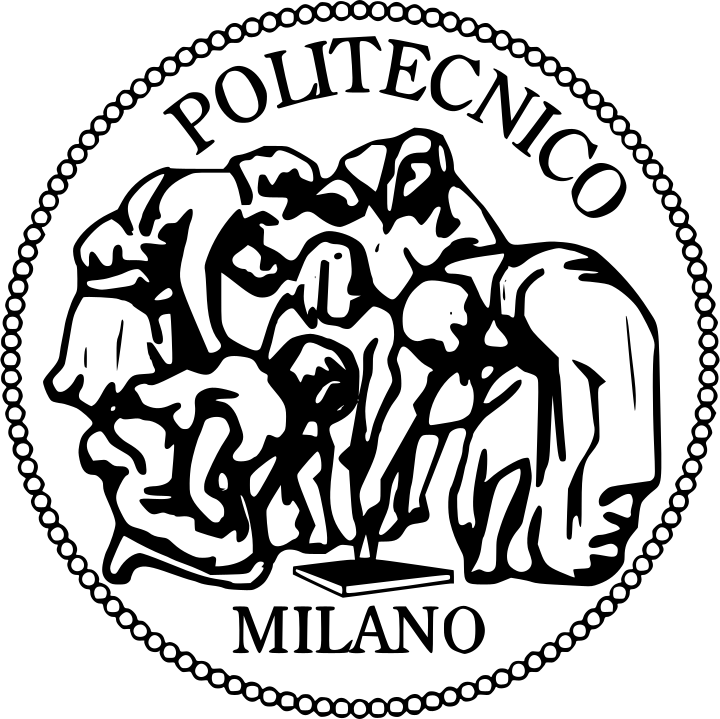
\includegraphics[width=0.3\textwidth]{title-page/logo-polimi}
\end{figure}
\vspace{0.5cm}
\par\end{center}

\begin{center}
\textbf{\LARGE{Analysis of a Vision-Based pose initialization algorithm for non-cooperative spacecraft on synthetic imagery}}\vspace{0.5cm}
\vspace{0.2cm}
\par\end{center}

\begin{center}
\textbf{D-Orbit}\\
\textit{in collaboration with}\\
\textbf{Space Missions Engineering Lab}
\end{center}\vspace{1.5cm}

\begin{flushleft}
\begin{tabular}{ll}
Relatore:  & Prof. Paolo LUNGHI\tabularnewline
Correlatore: & Dott. Ing. Aureliano RIVOLTA\tabularnewline
\end{tabular}\vspace{1.8cm}
\par\end{flushleft}

\begin{flushright}
\begin{tabular}{ll}
Tesi di laurea di: & \tabularnewline
Francescodario CUZZOCREA & Matr. 885016\tabularnewline
\end{tabular}\vspace{1.5cm}
\par\end{flushright}

\begin{center}
{\large{}Anno Accademico 2019-2020}{\large\par}
\par\end{center}

\end{titlepage}
\restoregeometry

\cleardoublepage{}

\begin{flushright}
\emph{To someone very special\ldots{}
}\cleardoublepage{}
\par\end{flushright}

\chapter*{Acknowledgments}

\thispagestyle{empty}%«È di cattivo gusto ringraziare il relatore. Se vi ha aiutato ha fatto solo il suo dovere» Umberto Eco, Come si fa una tesi di laurea
Ebbene si, alla fine cel'ho fatta anche io ad arrivare alla fine di questo lungo percorso universitario, iniziato in un soleggiato Settembre del 2009. Di questo devo molto a mio padre e mio fratello, che mi hanno supportato durante tutto questo tempo. Devo però ammettere che non sempre ho creduto di farcela, e cretedemi, non è solo una frase di circostanza, lo ho davvero creduto, sopratutto nei momenti più bui. Arrivare a questo punto non è stato per niente facile e mi è costato tanto, non solo in termini di salute fisica e mentale, ma anche e sopratutto in termini di rapporti umani. Ho conosciuto tante nuove persone che mi hanno aiutato non poco lungo questo percorso ma tante altre le ho perse a causa del mio essere costantemente preoccupato e spaventato per qualche esame, o, ultimamente, per la tesi. Fortunatamente però, sono riuscito a conoscere tante persone diverse che, chi più chi meno, mi hanno dato qualcosa e mi sono state vicine. In particolare, un pensiero speciale e la mia immensa gratitudine voglio dedicarli a Ilaria Cannizzaro e Jacopo Guarneri per il supporto tecnico e sopratutto morale che mi hanno fornito durante questa avventura trascorsa insieme in D-Orbit, specie mentre si discuteva di "rotazioni". Come non ringraziare inoltre il mitologico Flavio, che mi è sempre stato vicino, o come non ricordare Aureliano, Federico, Mattia, Umberto e Trevis che mi sono stati vicini sin dal lontano 2012, o anche Viviana e Andrea, sempre presenti per me quando la mia vita sentimentale andava a rotoli. Per non parlare dele famose "pause accademiche" di Stefano e Davide durante le lunghe sessioni di studio in biblioteca !! E' anche doveroso da parte mia dover ringraziare Alfonso e Benedetto, con i quali ho condiviso tutto il percorso della laurea Magistrale. A tutte queste persone conosciute in Università voglio dedicare il mio grazie per avermi sempre aiutato lungo tutto il mio percorso universitario. Ancora qualche riga voglio spenderla per mandare un pensiero ad Amro, Anas, Antonio, Emilio, Mayra e tutti i ragazzi che ho conosciuto in biblioteca durante la stesura finale di questo lavoro. Grazie a tutti voi ogni singola goccia di sudore spesa su questa tesi è stata accompagnata da un sorriso. Un debito ringraziamento voglio rivolgerlo a tutti i professori che in questi anni di Politecnico mi sono stati vicini, in particolare, i proff. Colombo, Quartapelle e Mantegazza meritano i miei ringraziamenti più sentiti per avermi aiutato a capire che tipo di strada intraprendere. 
\newpage
Infine, ma non certo ultimi per ordine di importanza, voglio ringraziare di cuore Cecilia e la sua famiglia per essermi stati vicini, per avermi sopportato ed avermi voluto bene negli anni passati.

\vspace{2cm}

Francescodario Cuzzocrea, \today, Milano\cleardoublepage{}

\chapter*{Abstract}

\thispagestyle{empty}
\cleardoublepage{}

\chapter*{Sommario}

\thispagestyle{empty}
\cleardoublepage\pagenumbering{roman}
\setcounter{page}{1}
\pagestyle{fancy}\tableofcontents{}\listoffigures
\listoftables
\listof{algorithm}{List of Algorithms}
\cleardoublepage\mainmatter
\renewcommand{\sectionmark}[1]{\markright{\thesection.\ #1}}
\renewcommand{\chaptermark}[1]{\markboth{\thechapter.\ #1}{}}

\chapter*{Introduction\label{chap:introduction}}

\addcontentsline{toc}{chapter}{Introduction}
\markboth{Introduction}{Introduction}%L’introduzione deve essere atomica, quindi non deve contenere né sottosezioni né paragrafi né altro. 
%Il titolo, il sommario e l’introduzione devono sembrare e e delle scatole cinesi, nel senso che lette in quest’ordine devono progressivamente svelare informazioni sul contenuto per incatenare l’attenzione del lettore e indurlo a leggere l’opera fino in fondo. 
%L’introduzione deve essere tripartita, non graficamente ma logicamente.

%Inquadramento generale
%La prima parte contiene una frase che spiega l’area generale dove si svolge il lavoro; una che spiega la sottoarea più specifica dove si svolge il lavoro e la terza, che dovrebbe cominciare con le seguenti parole «lo scopo della tesi è …», illustra l’obbiettivo del lavoro. 
%Poi vi devono essere una o due e frasi che contengano una breve spiegazione di cosa e come è stato fatto, e delle attività sperimentali, dei risultati ottenuti con una valutazione e degli a sviluppi futuri. 
%La prima parte deve essere circa una facciata e mezza o due.

%Breve descrizione del lavoro
%La seconda parte deve essere una esplosione della prima e deve quindi mostrare in maniera pi` esplicita l’area dove si svolge il lavoro, le fonti u bibliografiche pi` importanti su cui si fonda il lavoro in maniera sintetica u (una pagina) evidenziando i lavori in letteratura che presentano attinenza con il lavoro affrontato in modo da mostrare da dove e perché è sorta la tematica di studio. 
%Poi si mostrano esplicitamente le realizzazioni, le direttive future di ricerca, quali sono i problemi aperti e quali quelli affrontati e si ripete lo scopo della tesi. 
%Questa parte deve essere piena di citazioni bibliografiche e deve essere lunga circa 4 facciate.

%Struttura della tesi
%La terza parte contiene la descrizione della struttura della tesi ed è organizzata nel modo seguente. 
%«La tesi è strutturata nel modo seguente». Nella sezione due si mostra…, nella sezione tre si illustra… .

\chapter{State of Art\label{chap:first-chapter}}

\begin{quotation}
{\footnotesize
\noindent{\emph{``All models are wrong, but some are useful.''\\}
}
\begin{flushright}
George Box
\end{flushright}
}
\end{quotation}
\vspace{0.5cm}

\section{Host Company}
This thesis project was developed at D-Orbit.
D-Orbit is a New Space company with solutions convering the entire life-cycle of a space mission, including mission analysus and design, engineering, manufacturing, integration, testing, launch, mission control and end of life decommisioning.\\
The company's competitive advantage is in the versatility of its launch and deployement services that can me tailored to the customer's needs, from the launch procurement of a single spacecraft using standard deployment strategies to the precise deployment of a full constrallation with ION Satellite Carrier, a satellite dispenser developed and operated by D-Orbit.\\
ION Satellite Carrier can host any combination of CubeSat with a total volume of up to 48U and release them individually into distinct orbital slots, enabling delplyment schemes previously unavailable to spacecraft with no independet propulsion.\\
Committed to pursuin business modeal that are profitable, friendly for the environment, and socially beneficia, D-Orbit is the first certified B-Corp space company in the world.\\
Headquartered in Como, Italy, D-Orbit has subsidiaries in Lisbon, Portugal, Harwell, UK, and Washington DC, USA.\\

\section{Motivation}
Close range proximity operations between spacecrafts has been studied and discussed by space agencies and private companies since the early stages of space exploration, dating back to the Apollo program \cite{LangleyApollo}.\\
Since then we can find a wide range of missions where close-range proximity operations are in, like formation flying \cite{2001FormationFliying}  \cite{2009FormationFliying}, on-orbit servicing \cite{Zimpfer2005} \cite{Tatsch2006} \cite{FloresAbad2014} and active debris removal \cite{clerc2012astrium} \cite{Bonnal2013}.\\
Most of those missions were possible thanks to the presence of on-board crew or to the cooperativeness between spacecrafts.\\
A target space object is deemed cooperative if it is built to provide information suitable for the estimation of its distance and orientation in space with respect to the chaser spacecraft. Also, it can be be actively or passively cooperative depending on whether it interacts with a dedicated radio-link with the chaser spacecraft or not \cite{Opromolla2017}.\\
As regard to the new generation of space robotics missions such as debris removal and On-Orbit Servicing, proximity operations and docking are key-enabling capabilities for either repair, refuel or deorbit end-of-life and nonfunctional satellites \cite{2016Ventura}.\\
The main challenge when performing close-range navigation in actual on-orbit servicing and debris removal missions however is when the target spacecraft may be uncooperative.\\
This implies that the target spacecraft may not be equipped with an active communication link or identifiable markers such as light-emitting diodes or corner cube reflectors to help with computing the relative position and attitude of the active satellite (chaser) with respect to a uncooperative target space object \cite{2019phdSharma}.\\
Another important aspect, which comes out when dealing with uncooperative targets, is that debris or operating satellites to be serviced may have suffered physical damages as well as optical degradation of their surfaces due to the prolonged exposure to the space environment, thus appearing different than expected \cite{Opromolla2017}.\\
Thus, when operating in close-proximity the attitude and the motion of the target spacecraft must be estimated in autonomy by exploiting the sensors available on the servicer spacecraft.\\
With regards to the technological aspects, Electro-Optical (EO) sensors have been identified as the best option for relative navigation in the foredescribed scenario \cite{Opromolla2017} \cite{pesciolino}.\\
Either active Light Detection and Ranging (LIDAR) systems or passive monocular and stereo cameras can be used. The selection of the navigation sensor must consider the resources available on board in terms of mass, electrical and processing power, on one side, the mission scenario and the costs to be sustained for design and development of the satellite system, on the other side \cite{clerc2012astrium} \cite{pesciolino}.\\
As stated in \cite{Sharma2016} Monocular vision navigation has been identified as an enabling technology for present and future formation-flying and on-orbit servicing missions (namely PROBA-3 by ESA \cite{Casti2019}, PRISMA by OHB Sweden \cite{2013Damico}).\\
Monocular navigation on such missions relies on finding an estimate of the initial pose of the space resident object with respect to the camera, based on a minimum number of features from a 3D computer model and a single 2D image \cite{Sharma2016}.\\
In contrast to other state-of-the-art systems based on LIDAR or stero camera sensors, monocular navigation ensures rapid pose determination while offering some advantages such as lower hardware complexity, cost, weight and power consumption, possibility to be simultaneously used for supervised applications and a much larger operational range, not limited by the size of the platform \cite{Sharma2018} \cite{2016Ventura} \cite{pesciolino}.
However, the benefit of lower hardware complexity trades off with increased algorithmic complexity since a monocular sensor cannot provide direct
direct three-dimensional (3D) measurements about the target.\\
Moreover, monocular sensors can be less robust to adverse illumination conditions typical of the space environment \cite{Volpe2017} (e.g., saturation under direct Sun illumination, or absence of light during eclipse) \cite{pesciolino}.\\
The increasing challenges of space exploration and moreover the urgent need for debris removal to free slots in orbit and to avoid unwanted collisions is what mainly motivate this work.\\
The capability of being able to develop and test pose determination algorithm in fact will be a key factor for the overall success of new generation missions.\\
Furthermore this work is motivated also to give to the space community a FLOSS solution for simulating spaceborne imagery for computer vision alghoritm needs.\\

\section{Problem Statement}

\section{Structure of the Thesis}


\chapter{Problem setup\label{chap:second-chapter}}

\begin{quotation}
{\footnotesize
\noindent{\emph{``We are just an advanced breed of monkeys on a minor planet of a very average star. But we can understand the Universe. That makes us something very special.''\\}
}
\begin{flushright}
Stephen Hawking
\end{flushright}
}
\end{quotation}
\vspace{0.5cm}


\section{Synthetic Image Generation for Spaceborne Applications}

\subsection{Professional Solutions}

\subsubsection{ESA PANGU}

PANGU is a software developed in order to create synthetic planetary surface images, as much representative as possible, to aid the development of vision-based algorithms.\\
PANGU is a nice software which is ready to use. It's use is permitted for free for users working on an ESA project, while non-ESA users have to contact STAR-Dundee to purchase PANGU with technical support.\\
PANGU can also be integrated with proprietary or OSS simulation tools and it gives the possibility to correctly simulate a space camera in all its aspects (so focal lengths, and other relevant parameters of the image). It renders the images using OpenGL and it can use GPU cores to accelerate the rendering.

\subsubsection{Airbus Surrender}
SurRender is a software developed by Airbus Defense and Space. The software handles various space objects such as planets, asteroids, satellites and spacecraft.\\
It is capable of accommodating solar system-sized scenes without precision loss, and optimizes the ray tracing process to explicitly target objects. It can operate in real time mode to be coupled with  proprietary or OSS simulation tools and it gives the possibility to have an Hardware in The Loop simulation to test the responsiveness of the image processing subsystem. It gives the possibility to correctly simulate a space camera in all its aspects (so focal lengths, and other relevant parameters of the image). It parallelized and so can be ran on cloud platform to accelerate rendering times.\\

\subsection{Low-Cost Solutions}

\subsubsection{SPEED dataset: image generation using OpenGL}

\subsubsection{URSO dataset: image generation using Unreal Engine 4}

\section{Spaceborne Close-Proximity Relative Navigation}

\subsection{Pose estimation sensors}

\subsection{Pose estimation tecniques}




\chapter{Synthetic image generation\label{chap:third-chapter}}

\begin{quotation}
{\footnotesize
\noindent{\emph{``In math, you're either right or you're wrong.''\\}
}
\begin{flushright}
Katherine Johnson
\end{flushright}
}
\end{quotation}
\vspace{0.5cm}

\section{Mathematical Preliminaries}

\subsection{Reference Frames}
% copia paro paro quello che ha fatto il tizio nella tesi con i sistemi di riferimento

\section{Image generation}
The use of artificial images gives a complete control over the scene.\\
As stated in \cite{paolocorti}, the generated dataset should be as complete as possible in terms of metals and terrain features and illumination conditions.\\
A lack of realism in image generation can lead to incoherent results, not representative of real operative conditions and thus can lead to wrong results in terms of \acrshort{cv} algorithm tuning.\\
A particular care is then required in the image generation process.\\
For the purpose of this work, a new procedure for the generation of realistic images, representative of a dataset taken by a monocular navigation camera during a close-proximity approach to targeg \acrshort{sc} has been developed.\\
Without too much fantasy work, the procedure has been named Ray-traced Camera Simulation Tool for Spacecrafts (RCSTS).\\
Unsing the illustrated procedure, the user is able to create synthetic images of a target \acrshort{sc} given it's \acrshort{stl} model, by fine tuning all the properties of the materials composing the target \acrshort{sc}.\\
Since there could be also cases in which the Earth can be behind the target \acrshort{sc}, the developed tool is also able to simulate Earth's presence at any given location. The tool is also able to the simulate the the athmosphere of the Earth and the cloud layer \cite{jacopo}.\\

\subsection{Raytracing}
% copia paro paro jacopo

\subsubsection{What is raytracing}
% copia paro paro jacopo

\subsubsection{POVRay}
POVRay it is an opensource ray-tracing tool. It does not offer a nice GUI for modeling objects, like Blender, but it can be used as Blender rendering engine to be able to have a 3D modeling environment to model our objects. \\
POVRay has also been used by a different number of people doing research work in the space field to generate images, for example it has been used under the ESA LunarSim study to render images of lunar surfaces. It can also be extended to correctly simulate images of spacecraft. It is a powerful software which let us define surfaces and materials relevant properties such as reflectivity, diffraction, specularity and brillance. Those parameters can be fine tuned to obtain an image as realistic as possible, under certain limits.\\
POVRay can be scripted in order to be used in conjunction with other softwares.\\
Although does not let the user to add some sort of disturbance or noise to the generated images, those disturbances may be added by using some third party software such as MATLAB thanks to POVRay's ease of scriptability.\\
Up to a certain point, it also let us define some basic characteristic of the camera, such as the focal lengths, although it does not let us correctly simulate some other effects such as lens distorsions (which again, can be added using a third party software such as MATLAB).\\
POV-Ray major drawback are reported in \cite{pangufinal}, and are:
\begin{itemize}
    \item Only a Lambertian reflectance model is possible;
    \item A uniform surface albedo is used and realistic albedo values cannot used;
    \item The extended illumination source (sun) can be modelled only as an array of point light sources or as an area light, which is a suboptimal solution;
    \item Background lighting (starlight) is cannnot modelled;
    \item Earthshine cannot be easily modelled;
    \item POV-Ray can produceshigh quality images but rendering is slow as many minutes (sometimes hours) are required to produce a single image;
\end{itemize}
Despite those limitations POVRay can been used to produce synthetic space imagery with an acceptable degree of accuracy for \acrshort{cv} algorithm training.\\

\subsection{Environment Modeling}

\subsubsection{World Setup}
% storia delle terne

\subsubsection{Earth Modeling}
Earth modeling has been worked out in collaboration with Jacopo Guarneri.
Here will follow a brief review of how Earth has been modeled taken from \cite{jacopo}.
% copia paro paro jacopo

\paragraph{Cloud Layer}
% copia paro paro jacopo

\paragraph{Athmospheric Model}
% copia paro paro jacopo

\subsubsection{Light Modeling}
% copia paro paro jacopo

\subsection{Tango Spacecraft Modeling}
% copia un po franchiolla e un po il paper, devi solo dirgli come è fatto il satellite

\subsubsection{3D Model of the Spacecraft}

\subsubsection{Blender}

\subsubsection{POVRay}

\subsection{Camera Modeling}

\section{MATLAB integration}

\subsection{Random Attitude Image Generation}

\subsection{Pseudo-random Attitude Image generation}

\subsection{Caveats}


\chapter{The SVD architecture for pose initialization\label{chap:fourth-chapter}}

\begin{quotation}
{\footnotesize
\noindent{\emph{``Prediction is very difficult, especially if it's about the future.''\\}
}
\begin{flushright}
Niels Bohr
\end{flushright}
}
\end{quotation}
\vspace{0.5cm}

\section{Mathematical Preliminaries}

\subsection{Pinhole Camera Model}
%review of solution methods

\subsection{Image derivatives}
%review of solution methods

\subsection{The Hough Transform}
%review of solution methods

\subsection{Perspective-n-Point problem}
%review of solution methods

\section{Feature-based pose estimation implementation}

\subsection{Architecture}

\subsection{Image processing subsystem}

\subsubsection{Feature Detection}

\subsubsection{Feature Synthesis}

\subsubsection{Perceptual Grouping}

\subsection{Model Matching and Pose Determination}

\subsubsection{Feature Correspondence (?)}

\subsubsection{Pose Determination}




\chapter{Algorithm implementation\label{chap:fifth-chapter}}

\begin{quotation}
{\footnotesize
\noindent{\emph{``Most good programmers do programming not because they expect to get paid or get adulation by the public, but because it is fun to program.''\\}
}
\begin{flushright}
Linus Torvalds
\end{flushright}
}
\end{quotation}
\vspace{0.5cm}



\chapter{Results\label{chap:sixth-chapter}}

\begin{quotation}
{\footnotesize
\noindent{\emph{``If your experiment needs statistics, you ought to have done a better experiment.''\\}
}
\begin{flushright}
Ernest Rutherford
\end{flushright}
}
\end{quotation}
\vspace{0.5cm}


\chapter*{Conclusions\label{chap:conclusion}}

\addcontentsline{toc}{chapter}{Conclusions}
\markboth{Conclusions}{Conclusions}%Si mostrano le prospettive future di ricerca nell’area dove si è svolto il lavoro. 
%Nelle conclusioni si deve richiamare l’area, lo scopo della tesi, cosa è stato fatto, come si valuta quello che si è fatto e si enfatizzano le prospettive future e per mostrare come andare avanti nell’area di studio.
\bibliographystyle{plain}
\bibliography{bibliography}
\addcontentsline{toc}{chapter}{Bibliography}

\appendix

\chapter{First appendix\label{app:first-appendix}}




\chapter{Second appendix\label{app:second-appendix}}

\section{Kinematics}
In this section the kinematics representation used for the simulation will briefly be descripted. Two approach has been taken : 
\begin{itemize}
 \item [-] The DCM representation
 \item [-] The quaternion representation
\end{itemize}

\subsection{Direct Cosine Matrix}
The direct cosine matrix, or attitude matrix, gives the transformation of a vector from a reference frame $N$ to another reference frame $O$ : 

\begin{equation}
 \mathbf{r_{O}} = \mathbf{A_{ON}} \mathbf{r_{N}}
\end{equation}

So, if we consider the spacecraft body frame and the inertial frame, then we can write the relation between the two frames as : 

\begin{equation}
 \mathbf{r_{B}} = \mathbf{A_{B/N}} \mathbf{r_{N}}
\end{equation}

As it is demonstrated in Ref. \cite{Markley2014}, we can express the time dependence of the attitude matrix by writing the rotation from the body frame to the inertial frame as : 

\begin{equation}
 \dot{A}_{B/N}= - [\omega_{B/N} \times]A_{B/N} 
\end{equation}

where $[\omega_{B/N} \times]$ is the skew-symmetric cross product matrix containing the components of the angular velocity vector : 

\begin{equation*}
 \mathbf{[\omega \times]} =
                                \begin{bmatrix}
                                    0 & -\omega_{B/N_{3}} & \omega_{B/N_{2}} \\
                                    \omega_{B/N_{3}} & 0 & -\omega_{B/N_{1}} \\
                                    -\omega_{B/N_{2}} & \omega_{B/N_{1}} & 0
                                \end{bmatrix}
\end{equation*}

Thus, by integrating this relation, we can get full attitude at every iteration.

\subsection{Quaternions}
Quaternions are another way to parametrize the attitude of a rigid body in space. They are commonly used for control purpose due to the fact that they don't have kinematics singularities.
A quaternion is a four-component vector with some additional operations defined on it. A quaternion $\mathbf{q}$ has a three-vector part $\mathbf{q_{1:3}}$ and a scalar part $q_{4}$ : 

\begin{equation*}
 \mathbf{q} =
                                \begin{bmatrix}
                                    q_{1}\\
                                    q_{2}\\
                                    q_{3}\\
                                    q_{4}\\
                                \end{bmatrix}
\end{equation*}

The kinematic equation for the quaternion can be written as :

\begin{equation}
 \label{eq:quaternion}
 \dot{q} = \frac{1}{2} \mathbf{\varXi(\mathbf{q})} \mathbf{\omega_{B/N}}
\end{equation}

where $\mathbf{\varXi(\mathbf{q})}$ is defined as 

\begin{equation*}
 \mathbf{\varXi(\mathbf{q})} =
                                \begin{bmatrix}
                                   q_4 & -q_3 & q_2\\
                                   q_3 & q_4 & -q_1\\
                                  -q_2 & q_1 & q_4\\
                                  -q_1 & -q_2 & -q_3\\
                                \end{bmatrix}
\end{equation*}

By integrating Eq. \ref{eq:quaternion} can get the full attitude at every iteration in terms of quaternion.

\section{Dynamics}
\subsection{Euler Equations}
The dynamics of a rigid body which is tumbling into space can be modeled by mean of the well known Euler equations : 

\begin{equation}
  \mathbf{\omega_B} = \mathbf{(I_B)}^{-1} [\mathbf{L_B} - \mathbf{\omega_b}  \wedge (\mathbf{I_B} \mathbf{\omega_b})
\end{equation}

where \textbf{$\omega_B$} is the angular velocity vector of the spacecraft in body frame, \textbf{$I_B$} is the inertia tensor of the spacecraft in body frame and \textbf{$L_B$} are the external torques acting on the spacecraft due to  external disturbances and control torques.

\subsection{Environmental Disturbances} \label{sec:disturbances}
The external disturbances acting on spacecraft placed in a LEO orbit are basically four and are due to :

\begin{itemize}
  \item[-] Gravity Gradient
  \item[-] Magnetic Field 
  \item[-] Solar Radiation Pressure
  \item[-] Aerodynamic Drag
\end{itemize}

Details about how those torques have been mathematically modeled will be given in the following sections.

\subsubsection{Gravity Gradient}
Any non-symmetrical rigid body in a gravity field is subject to a gravity-gradient torque.
If we consider a rigid spacecraft, the torque due to the gravity gradient about the spacecraft's center of mass can be modeled as :

\begin{equation}
 \mathbf{L_{gg}} = \frac{3 \ mu}{r^3} \mathbf{n} \wedge (\mathbf{I} \ \mathbf{n})
\end{equation}

where $\mu$ is the Eart's gravitational constant, $\textbf{r}$ is the radius vector from the center of the Earth, thus $r \equiv \Vert{\textbf{r}}\Vert$, $\textbf{I}$ is the inertia tensor in body frame and $\textbf{n}$ is the body frame representation of a nadir-pointing unit vector.\\
Further details about the model can be found in reference \cite{Markley2014}.

\subsubsection{Earth's Magnetic Field}
The torque generated by a magnetic dipole $\textbf{m}$ in a magnetic field $\textbf{B}$ is

\begin{equation}
 \mathbf{L_{mag}} = \mathbf{m} \wedge \mathbf{B}
 \label{eq:magfield}
\end{equation}

where $\mathbf{B}$ is the magnetic field in the body frame.
The most basic source of a magnetic dipole is a current loop. A current of I amperes flowing in a planar loop of area A produces a dipole moment of magnitude m=IA in the direction normal to the plane of the loop and satisfying a right-hand rule.
When $\textbf{m}$ is in $Am^2$ and the magnetic field is specified in Tesla, Eq. \ref{eq:magfield} gives the torque in $Nm$. If there are N turns of wire in the loop, the dipole moment has magnitude m=NIA (such as the case of a magnetic torquer).
To model $\textbf{B}$ either the full IGRF model or the simple dipole model can be used.\\
For what concerns this work, the full IGRF model truncated to the 10th order has been used. Further details about the model can be found in reference \cite{Davis2014}

\subsubsection{Solar Radiation Pressure}
Solar radiation pressure acting on the surfaces of the spacecraft causes a disturbance torque that in general, cannot be neglected for orbits higher than \SI{800}{\kilo\meter}, so it has been taken into account in this work.
The SRP torque is zero zero when the spacecraft is in the shadow of the Earth or any other body, of course.
To take into account the effect of solar radiation pressure on the spacecraft, the spacecraft's surface can be modeled as a collection of $N$ flat plates of area $S_{i}$, outward normal $\mathbf{n_{b}}$ in the body coordinate frame, specular reflection coefficient $\rho_s$, diffuse reflection coefficient $\rho_{d}$ and absorption coefficient $\rho_{a}$; those coefficients must sum to unity.
For what concerns this work, only $\rho_s$ and $\rho_d$ have been considered, since all the absorbed radiation is emitted as thermal radiation,  although not necessarily at the same time or from the same surface as its absorption.
For an accurate modeling of thermal radiation we must also known the absolute temerature and the emissivity of each surface.
We can define the spacecraft-to-Sun unit vector in the spacecraft's body frame as : 

\begin{equation}
 \mathbf{s_b} = \mathbf{A_{B/N}} \mathbf{s_i}
\end{equation}

where $\mathbf{A_{B/N}}$ is the attitude matrix and $\mathbf{s_i}$ is the spacecraft-to-Sun unit vector in the GCI frame.
We can define the angle between the Sun vector and the normal exiting from the normal to the i-th plate as : 

\begin{equation}
 cos(\theta_{SRP}^{i}) = \mathbf{n}_{B}^{i} \cdot \mathbf{s_b}
\end{equation}

The SRP force on the i-th plate can be expressed as : 

\begin{equation}
 \mathbf{F}_{SRP} = - P_{Sun}A_{i}\left[ 2\left( \frac{\rho_{d}^{i}}{3} + \rho_{s}^{i}cos(\theta_{SRP}^{i}) \right) \mathbf{n}_{B}^{i} + (1 -\rho_{s}) \mathbf{s_b} \right] max(cos(\theta_{SRP}^{i}),0)
\end{equation}

where $P_{Sun}$ is the solar radiation pressure.
The Solar radiation pressure torque acting on the spacecraft is then given by :

\begin{equation}
    \mathbf{L}_{SRP}^{i} = \sum\limits_{i=1}^n  \mathbf{r}_{i} \times \mathbf{F}_{SRP}^{i} 
\end{equation}

where $\mathbf{r}_{i}$ is the vector from the spacecraft center of mass to the centre of pressure of the SRP on the i-th face.
In this formulation we are not considering the albedo radiation coming from the Earth and from the Moon.
Further details on how the solar radiation pressure, the spacecraft-to-Sun unit vector and the eclipse condition have been modeled can be found in reference \cite{Markley2014}.

\subsubsection{Aerodynamic Drag}
Aerodynamic torque is generally computed by modeling the spacecraft as a collection of $N$ flat plates of area $A_i$ and outward normal unit vector $\mathbf{n_{B}}$ expressed in the spacecraft body-fixed coordinate system. The torque depends on the velocity of the spacecraft relative to the atmosphere, which is not simply the velocity of the spacecraft in the GCI frame, because the atmosphere is not stationary in that frame.
The most common assumption is that the atmosphere co-rotates with the Earth. The relative velocity in the GCI frame is then given by : 

\begin{equation}
 \mathbf{v_{relI}} =  \mathbf{v_I} + [\mathbf{\omega_{\earth} \times}] \mathbf{r_I}
\end{equation}

where $\mathbf{r_I}$ and $\mathbf{v_I}$ are the position and velocity of the spacecraft expressed in the GCI frame. 
The Earth's angular velocity vector is $\mathbf{\omega_{\earth}} = \omega_{\earth}[0 0 1]'$ with $\omega_{\earth}$ = \SI{0.000072921158553}{\radian/\second}.
The velocity in the body frame is the computed as : 

\begin{equation}
 \mathbf{v_{relB}} = \mathbf{A_{B/N}}   \begin{bmatrix} \dot{x} + \omega_{\earth} y \\ \dot{y} - \omega_{\earth} x \\ \dot{x} \end{bmatrix}
\end{equation}

The inclination of the i-th plate WRT the relative velocity is given by : 

\begin{equation}
 cos(\theta_{aero}^{i}) = \frac{\mathbf{n}_{B}^{i} \cdot \mathbf{v}_{rel\ B}}{\norm{\mathbf{v}_{rel}}}
\end{equation}

The aerodynamic force on i-th plate in the flat plate model is

\begin{equation}
 \mathbf{F}_{aero}^{i} = - \frac{1}{2} \rho C_{D} \norm{\mathbf{v}_{rel}} \mathbf{v}_{rel_{} B}\ S_{i}\ max(cos(\theta_{aero}^{i}),0)
\end{equation}

where $\rho$ is the atmospheric density, and $C_D$ is the drag coefficient.  
$\rho$ can be modeled by mean of the well known exponential decaying model for the atmospheric density :

\begin{equation}
 \rho = \rho_{0} e^{(-(h-h_{0})/H)}
\end{equation}

where $\rho_{0}$ and $h_{0}$ are reference density and height, respectively, $h$ is the height above the ellipsoid and $H$ is the scale height, which is the fractional change in density with eight.
The value of $\rho_{0}$, $h_{0}$  and $H$ changes with $h$. 
The values used to perform the simulation are the one given in \cite{Markley2014}.
The actual torque due to the aerodynamic drag can be computed as : 

\begin{equation}
 \mathbf{L}_{aero}^{i} = \sum\limits_{i=1}^n  \mathbf{r}_{i} \times \mathbf{F}_{aero}^{i}
\end{equation}

where $n$ is the number of faces and $\mathbf{r}_{i}$ is the vector from the spacecraft center of mass to the center of pressure on the $i$ th face.


\chapter{Third appendix\label{app:third-appendix}}


\cleardoublepage
\end{document}
